%%%%%%%%%%%%%%%%%%%%%%%%%%%%%%%%%%%%%%%%%%%%%%%%%%%%%%%%%%%%%%%%%%%%%%%%%%%%%%%%%%%%%%%%%%%%%%%%%%%%%%%%%%%%%%%%%%%%%%%%%
\subsection{Why WA Persists on Commodity SSDs}\label{sec:ssdwaexists}

\revision[R2.W2]{\module{Standard SSDs can exhibit high WAF.}
When standard SSDs are used instead of ZNS, the same write pattern can incur high SSD WAF due to internal GC.
Although SSD-level WAF reduction has been widely studied, our prior work shows that modern enterprise SSDs still exhibit high WAF even under simple skewed workloads~\cite{ssdiq}.
Thus, even when DB WAF is reduced with our prior optimizations, excessive SSD WAF can negate overall gains.

\module{SSD WAF is shaped by DB GC behavior.}
For a fixed device, the dominant factor influencing SSD WAF is the write pattern generated by the DBMS~\cite{flashalloc}.
In our setting, DB GC shapes this pattern in three ways.
First, GC trigger points determine the SSD’s effective OP space: higher fill factors leave less OP space and increase SSD WAF. 
Second, DB GC granularity affects whether pages from the same zone remain colocated on SSD blocks.
Third, victim-zone selection determines which zones are rewritten together, influencing internal write clustering.
Together, these choices define the write stream the SSD receives and thus directly affect SSD WAF.


\module{DBMS has more control than SSDs to mitigate SSD WAF.}
Although the write pattern is explicit at the DBMS layer, SSDs have no visibility into it~\cite{DBLP:journals/pomacs/LangeNY25}, making SSD-side mitigation difficult.
Prior work attempts to infer workload characteristics inside the SSD~\cite{DBLP:journals/pomacs/LangeNY25,DBLP:journals/cacm/LangeNY23,DBLP:journals/pvldb/KangCOL20}, but such inference is costly and inherently imperfect.
We take the opposite approach: the DBMS, which has full workload knowledge~\cite{SNIA_SDC_2025_TotalCostAndPerformanceOfSSDs}, guides writes to reduce SSD WAF directly.
By understanding SSD placement and GC behavior, the DBMS can \emph{proactively} structure writes to avoid GC-induced amplification.
}

\subsection{Aligning DB and SSD GC Granularity}\label{sec:gcgranularity}
A key insight available to the DBMS is that writes to the same zone share similar deathtimes.
This section explains why aligning DB and SSD GC granularity is the first step toward reducing SSD WAF using this insight.
We then show how the upper bound of SSD GC granularity can be inferred from ZNS-like patterns.
When an SSD features FDP, the Reclaim Unit size directly provides this value.

\module{Background: placement and GC granularity of SSDs.}
A superblock is the SSD’s primary append unit, formed by grouping erase blocks across planes and dies to exploit internal parallelism.
When a stream of page writes arrives, the SSD controller appends them to the active superblock and maps Logical Block Addresses (LBAs) to Physical Block Addresses (PBAs) after persistence.
Once the superblock fills, the SSD switches to a new one.
As the device fills and free space becomes scarce, GC reclaims space at a vendor-specific granularity, 
which may range from a single erase block to an entire superblock~\cite{SSDhistory,lerner2024principles}.

\begin{figure}[t]
    \centering
    \begin{minipage}[b]{0.49\linewidth}
        \centering
        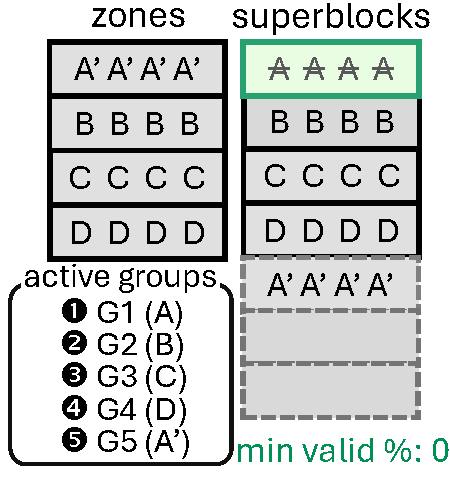
\includegraphics[width=0.7\linewidth]{figures/gcunitsize0.pdf}
        \caption{Zone size matches superblock size}
        \label{fig:gcunit0}
    \end{minipage}\hfill
    \begin{minipage}[b]{0.49\linewidth}
        \centering
        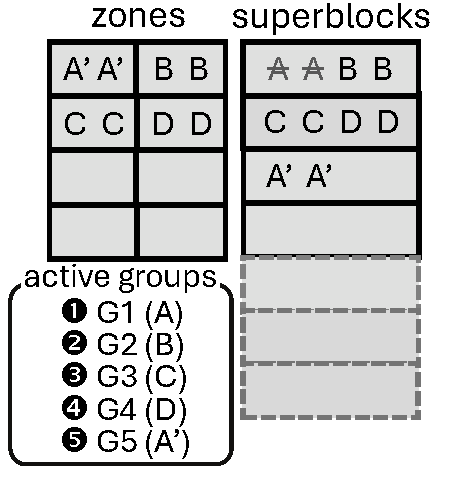
\includegraphics[width=0.7\linewidth]{figures/gcunitsize1.pdf}
        \caption{Zone size is smaller than superblock size}
        \label{fig:gcunit1}
    \end{minipage}
\end{figure}



\module{Estimating physical placement inside SSDs: simple case.}
To reason about physical placement, we use a simplified example that reflects general SSD behavior.
Suppose the SSD has seven superblocks, each holding four SSD pages (4~KiB), with three reserved as OP space, as shown in \cref{fig:gcunit0}.
The DBMS runs on top of the SSD, and DB GC is invoked when SSD capacity is nearly exhausted (four zones) and stops after reclaiming a target amount of space.
An \emph{SSD page} here refers to a 4~KiB LBA offset.
SSD pages belonging to the same DB zone share the same label.
For example, if zone~A spans LBAs 0--16~KiB, its first four SSD pages are labeled \emph{A}.
An \emph{active zone} is a zone currently receiving appends, and multiple active zones form an \emph{active group}.
A new zone becomes active only after all zones in the current group are fully written.
Thus, the number of zones the DBMS appends simultaneously determines the number of active zones and the size of the active group.

\module{Writes from the same zone share the same deathtime.}
\cref{fig:gcunit0} illustrates the case where only one zone is active and the zone size matches the superblock size.
When zone~A is appended (active group \ding{182}), its four writes (i.e., A pages) are placed together in the first superblock.
Later, when DB GC rewrites zone~A (active group \ding{186}), the new A' pages are written to the fifth superblock,
invalidating all old A pages in the first superblock and leaving it fully invalidated.

\module{DB GC granularity controls deathtime clustering.}
However, if the zone size is smaller than the superblock size, the first superblock does not become fully invalid.
In \cref{fig:gcunit1}, the zone size is half a superblock.
Even if the same active group is used as in \cref{fig:gcunit0}, SSD pages from zones A and B are interleaved within a superblock, mixing pages with different deathtimes~\cite{DBLP:conf/osdi/YangPGTS14}.
When DB GC rewrites zone~A (\ding{186}), only half of the superblock’s pages are invalidated.

\module{Aligning GC unit size to place writes with the same deathtime.}
These examples reveal two insights: (1) a write stream whose size matches the superblock is internally placed and GCed together, 
and (2) writes from a single zone form such a stream only when the DB and SSD GC units are aligned.
Thus, the SSD’s GC unit size determines the largest region whose pages can share the same deathtime and yield empty superblocks.
From the DBMS’s perspective, this maximum size can be used directly as the zone size.

\module{Optimization: using RU size (FDP-enabled SSDs).}
Standard SSDs usually do not expose the SSD GC granularity.
Fortunately, FDP explicitly exposes the SSD’s Reclaim Unit (RU), the smallest granularity at which SSD GC operates~\cite{SSDhistory}.
With this information, we can set the database’s zone size to match the RU size, ensuring that writes are aligned to the SSD’s internal GC boundaries.

\revision[R2.D7]{
\module{Optimization: using inferred GC unit size (standard SSDs).}
For SSDs without FDP, we approximate the upper bound of the SSD’s GC unit size using a ZNS-like write pattern.
With a single active zone, SSD WAF converges to~1 once the zone size meets or exceeds the internal append unit (\cref{fig:gcunit0}).
Thus, by gradually increasing the zone size and observing when WAF first reaches~1, we estimate this upper bound.

\module{Inferring the GC unit size with a ZNS-like pattern.}
We validate this approach on six enterprise SSDs, including two FDP-enabled devices, by varying the database zone size:
\begin{center}
  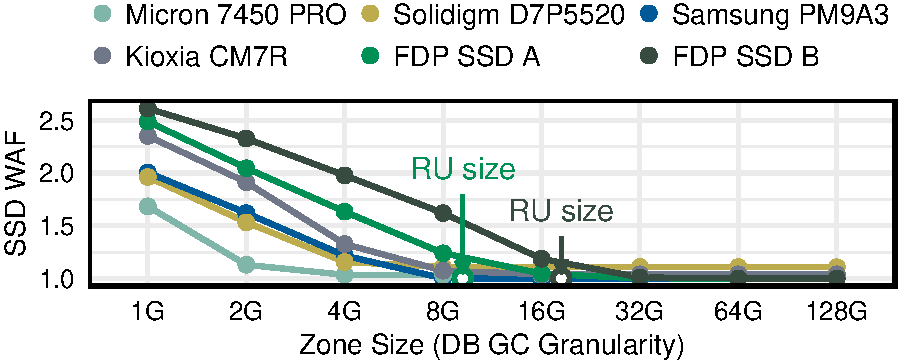
\includegraphics[width=0.8\linewidth]{figures/blocksz.pdf}
\end{center}
\noindent
On FDP-enabled SSD~A, WAF drops to~1 at a 16\,GB zone size, consistent with its 8{,}496\,MB RU size lying between 8 and 16\,GB.
The same holds for FDP-enabled SSD~B, whose RU size is slightly above 16\,GB.
Across the other four enterprise SSDs, the inferred GC unit size typically falls between 4\,GB and 8\,GB.
Thus, the zone size at which WAF reaches~1 provides a practical upper bound on SSD GC granularity.
Although approximate, this bound is sufficient to avoid mixing DB writes with different deathtimes.
}
\revision[R3.D3]{For SSDs without OCP commands or FDP support, we recommend using a 32\,GB zone size as a safe upper bound.
Alternatively, one can indirectly estimate SSD WAF by checking whether the throughput goes down~\cite{ssdiq}. }


% \module{Unifying SSD and DB GC granularity size.}
% If the SSD supports FDP, the RU size exposed by the interface can be directly used as the database zone size.
% Otherwise, the zone size should be determined by running a ZNS-like write pattern with increasing sizes until SSD WA converges to 1.
% This alignment ensures that the NoWA pattern remains effective, even when the host utilizes 100\% of the SSD space.
% % To our knowledge, this is the first work to propose a write pattern that fully eliminates SSD WA under full-capacity usage.
% % File systems and other storage systems built on SSDs can also adopt this approach to minimize internal WA.

